\usepackage{lmodern, ragged2e, CJKutf8, booktabs, subfigure, graphicx, algorithm, algorithmicx, algpseudocode, amsmath, amssymb, amsthm, amsfonts, mathtools, multirow}
\usepackage[style=phys]{biblatex}
\addbibresource{bibliography.bib}
\renewcommand{\footnotesize}{\tiny}
\makeatletter
\@newctr{footnote}[page]
\makeatother
\usetheme{CambridgeUS}
\renewcommand{\raggedright}{\leftskip=0pt \rightskip=0pt plus 0cm}



\definecolor{TEC blue}{RGB}{0, 32, 159}
\newcommand{\hl}[1]{{\textcolor{TEC blue}{#1}}}

% Theme setup
\titlegraphic{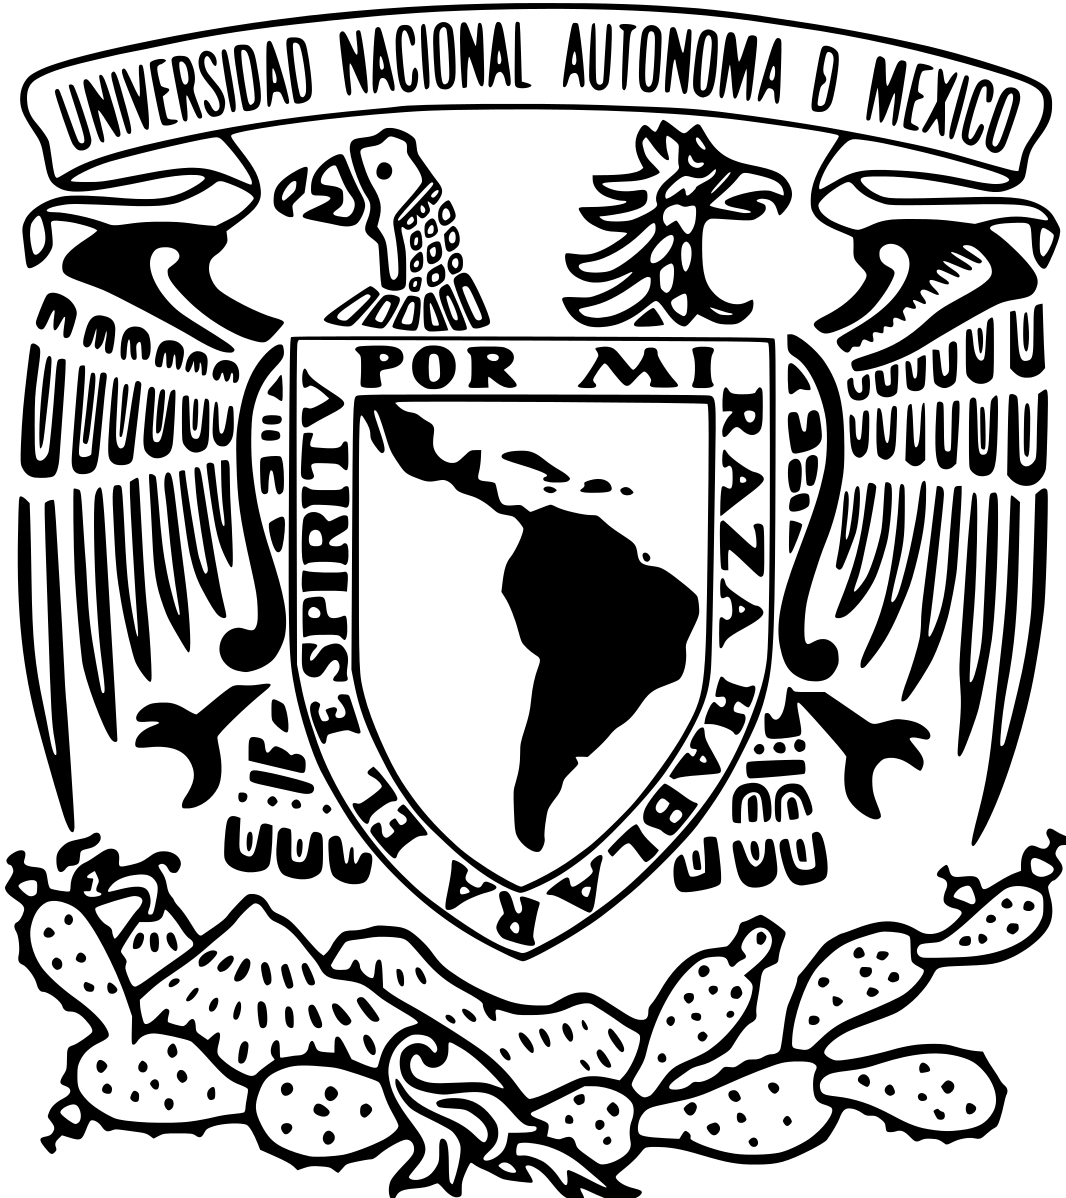
\includegraphics[scale=0.07]{Figures/logounam.png}}

% \makeatletter
\setbeamertemplate{headline}{%
\leavevmode%
  \hbox{%
    \begin{beamercolorbox}[wd=\paperwidth,ht=2.5ex,dp=1.125ex]{palette quaternary}%
    \insertsectionnavigationhorizontal{\paperwidth}{}{\hskip0pt plus1filll}
    \end{beamercolorbox}%
  }
}
\setbeamertemplate{footline}{\hspace*{2ex} \insertshortauthor \hfill \textcolor{TEC blue}{\insertshorttitle} \hfill \textbf{\insertframenumber{}} / \inserttotalframenumber \hspace*{2ex}}

\setbeamercolor{item projected}{bg=TEC blue}
\setbeamertemplate{enumerate items}[default]
\setbeamercolor*{enumerate item}{fg=TEC blue}

\setbeamertemplate{navigation symbols}{} 
% \setbeamertemplate{footline}[\insertshorttitle frame number]
\setbeamertemplate{bibliography item}[text]
\setbeamertemplate{theorems}[numbered]

\setbeamerfont{title}{series = \bfseries, parent = structure}
\setbeamerfont{frametitle}{series = \bfseries, parent = structure}
\setbeamerfont{headline}{series = \bfseries, size = \tiny, parent = structure}

\setbeamercolor{title}{fg = white, bg = TEC blue}
\setbeamercolor{frametitle}{fg = white, bg = TEC blue}
\setbeamercolor{structure}{fg = TEC blue}
\setbeamercolor{section in head/foot}{fg = black, bg = TEC blue!40}
\setbeamercolor{subsection in head/foot}{fg = black, bg = TEC blue!20}

\setbeamercolor{block title}{use=structure,fg=white,bg=structure.fg!75!black}
\setbeamercolor{block body}{parent=normal text,use=block title,bg=TEC blue!20} %block title.bg!10!bg}
\makeatletter
\def\th@mystyle{%
    \normalfont % body font
    \setbeamercolor{block title example}{bg=orange,fg=white}
    \setbeamercolor{block body example}{bg=orange!20,fg=black}
    \def\inserttheoremblockenv{exampleblock}
  }
\makeatother
\theoremstyle{mystyle}
\newtheorem*{remark}{Remark}

\usepackage{tikz}
\setbeamertemplate{background}{\tikz[overlay,remember picture]\node[opacity=0.05]at (current page.center){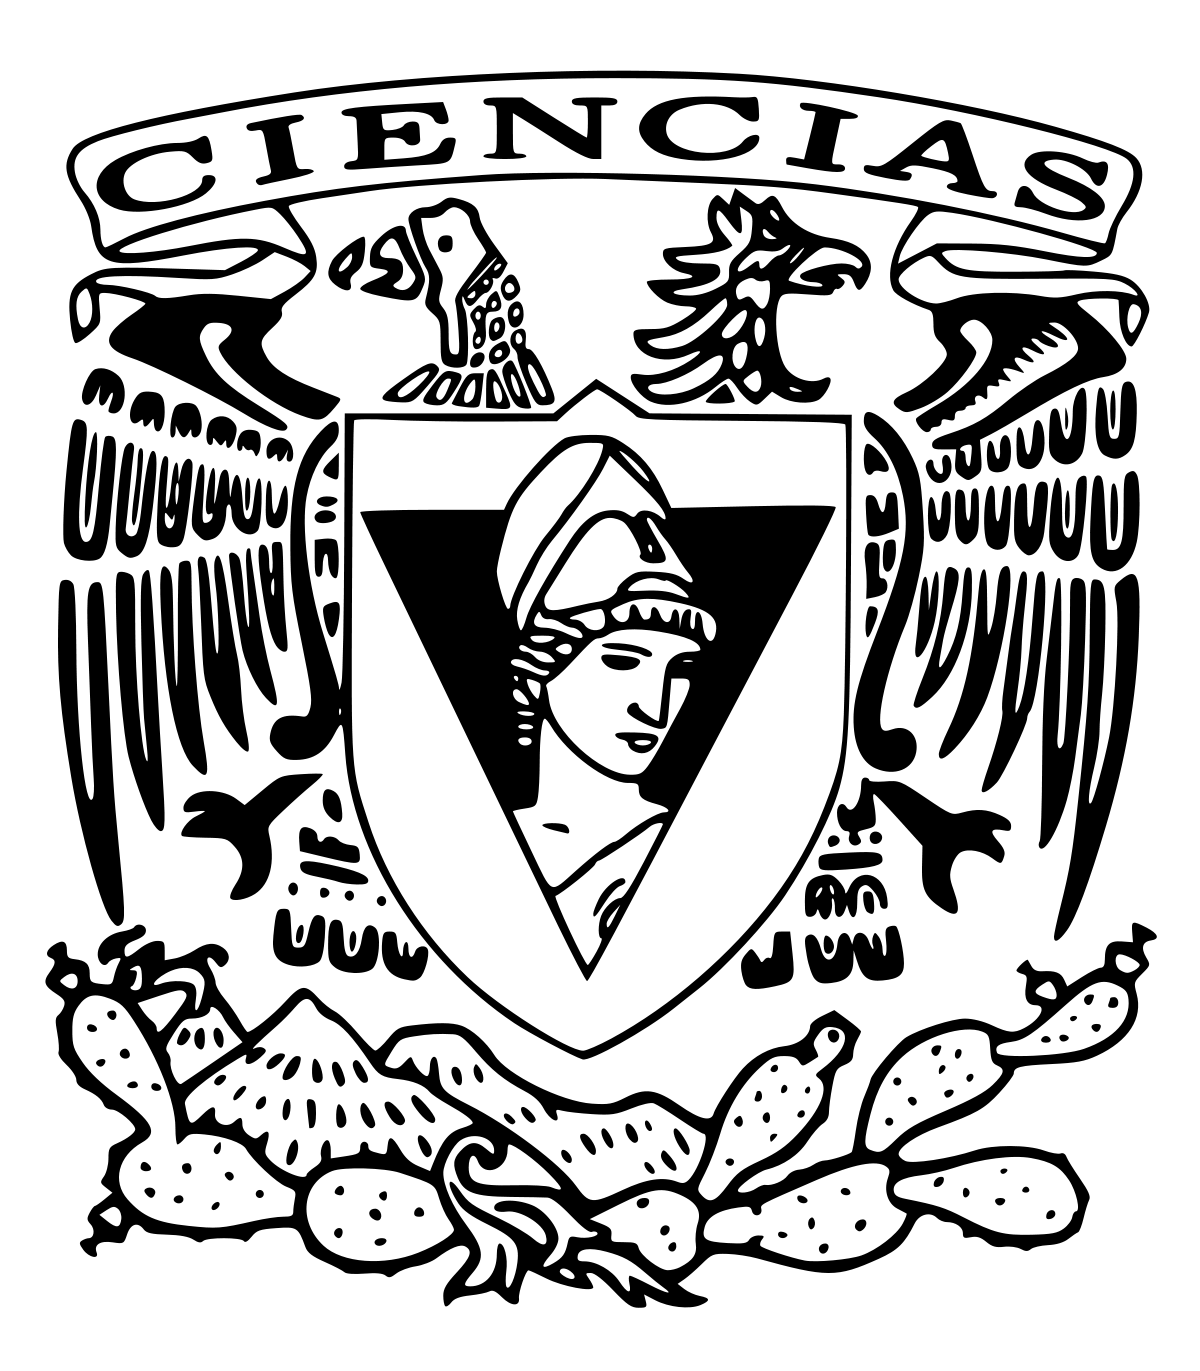
\includegraphics[width=6cm]{Figures/logociencias.png}};}


\newcommand{\maketitleandtoc}{%
{%
    \setbeamertemplate{headline}{}%
    \setbeamertemplate{footline}{}%
    \begin{frame}[noframenumbering]%
        \titlepage%
    \end{frame}%
    \begin{frame}[noframenumbering]%
        \frametitle{Contenido}%
        \tableofcontents%
    \end{frame}%
}}

\newcommand{\noheadfoot}[1]{%
    {%
        \setbeamertemplate{headline}{}%
        \setbeamertemplate{footline}{}%
        {#1}
    }
}